\chapter{Resultados e discussão}\label{cap:resultados}
\rubricaComunicacao
\section{Séries temporais finais da campanha}
A campanha final abrange 25h29min27s de dados de chegada; no subconjunto de 3.080 telemetrias logicamente únicas, a temperatura variou de 26,9 a 36,9~\si{\celsius}, e a umidade relativa de 34\% a 73\%. As Figuras~\ref{fig:temp-final} e~\ref{fig:ur-final} apresentam somente pontos medidos, sem interpolar temporalmente o período da queda de Wi-Fi. Os eventos de intervenção são marcados no eixo de tempo pelo diário; a escala representa hora local (UTC-3). Os gráficos não são certificados metrológicos do DHT11 e não demonstram generalização espacial do cômodo.
\begin{figure}[H]\centering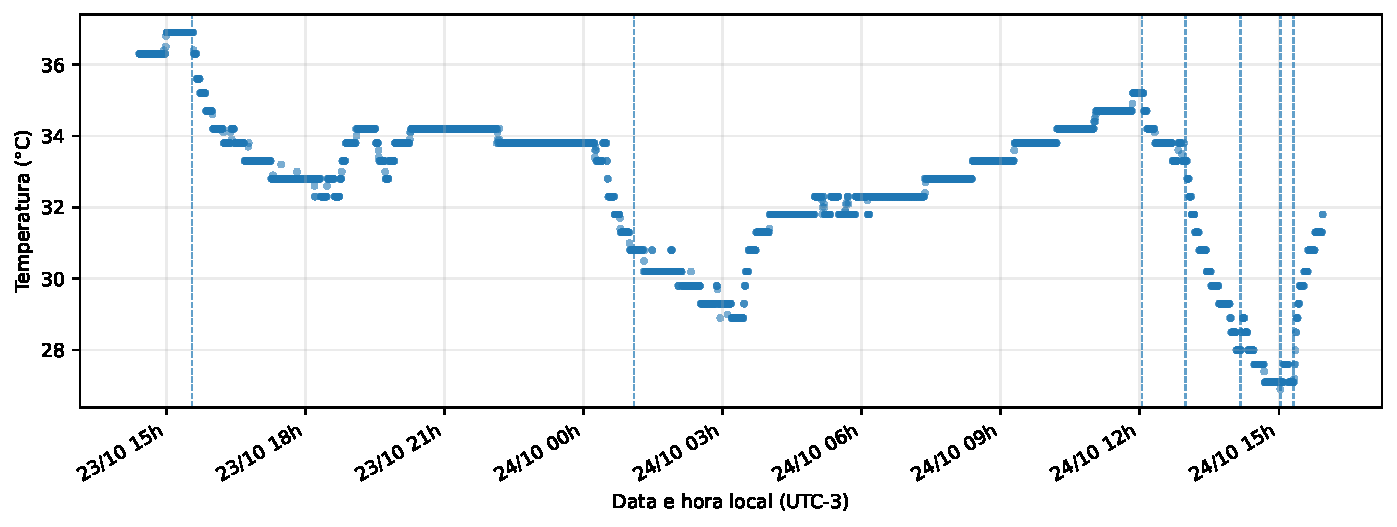
\includegraphics[width=\textwidth]{figuras/temperatura_serie_final.pdf}\caption{Série final de temperatura com intervenções indicadas por linhas verticais.}\label{fig:temp-final}\fonte{\texttt{dados/mensagens.csv}, telemetrias únicas, horário de aquisição válido ou recepção no único ponto com \texttt{ts:null}.}\end{figure}
\begin{figure}[H]\centering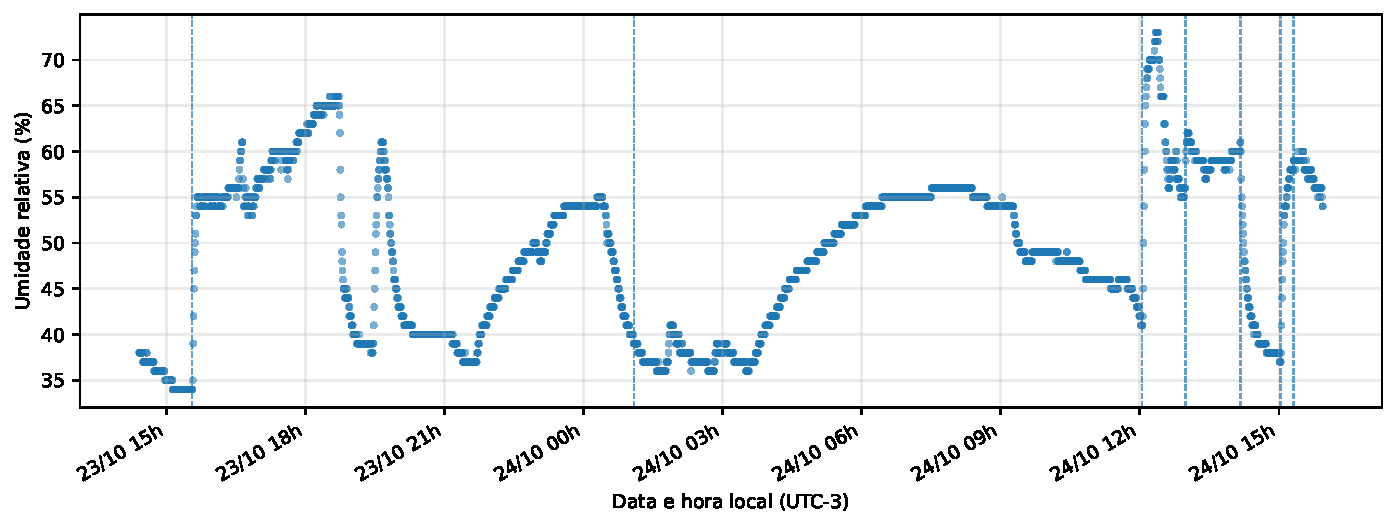
\includegraphics[width=\textwidth]{figuras/umidade_serie_final.pdf}\caption{Série final de umidade relativa, sem interpolação de lacunas.}\label{fig:ur-final}\fonte{CSV final e diário, 23--24/10/2026.}\end{figure}
\section{Umidificação isolada: primeira intervenção}
Em 23/10, às 15h33, o umidificador foi acionado manualmente. Duas janelas adjacentes de 30~min (15h03--15h33, antes; 15h33--16h03, após) contiveram 60 amostras válidas cada. A umidade média passou de 34,15\% para 52,87\% (diferença de +18,72 pontos percentuais), enquanto a temperatura média caiu de 36,90 para aproximadamente 35,22~\si{\celsius} (diferença de $-1,68$~\si{\celsius}). Esses contrastes são descritivos e associados temporalmente ao evento, sem grupo de controle, randomização nem estabilização do ambiente.
\begin{figure}[H]\centering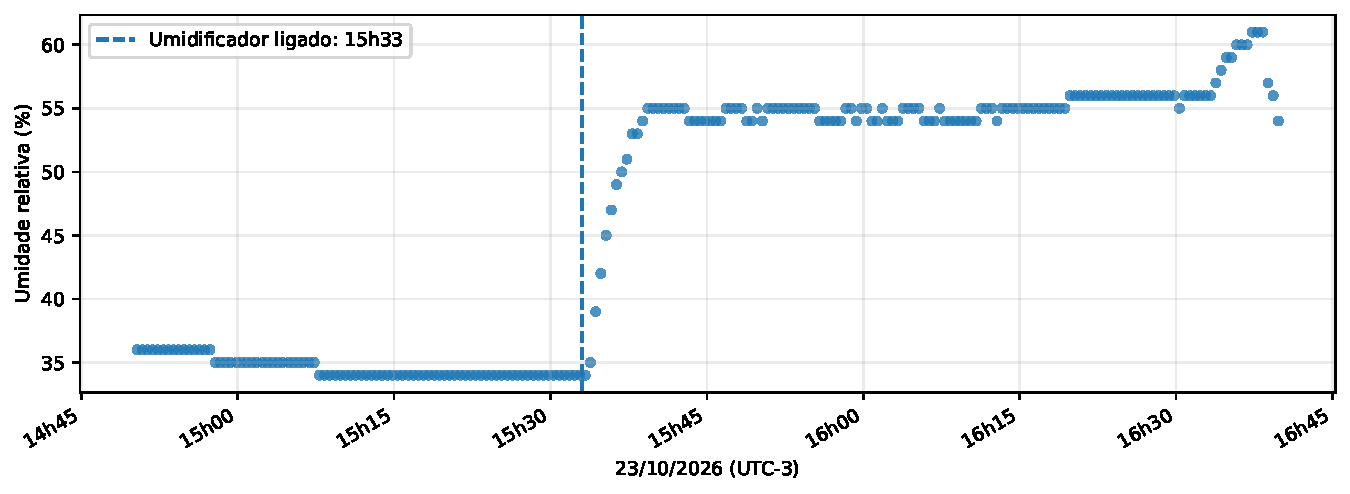
\includegraphics[width=.95\textwidth]{figuras/evento_umidificador_final.pdf}\caption{Umidade relativa na janela próxima ao acionamento de 23/10 às 15h33.}\fonte{CSV final, janelas explicitadas no texto.}\end{figure}
\begin{table}[H]\centering\caption{Comparação de 30 min antes e depois do primeiro acionamento}\label{tab:prepos}\footnotesize
\begin{tabular}{@{}L{6.3cm}R{2.45cm}R{2.45cm}R{2.7cm}@{}}\toprule
Variável&Antes ($n=60$)&Depois ($n=60$)&Diferença\\\midrule
Umidade relativa média (\%)&34,15&52,87&+18,72 p.p.\\
Temperatura média (\si{\celsius})&36,90&35,22&$-1,68$~\si{\celsius}\\\bottomrule\end{tabular}\fonte{Cálculo sobre CSV final; médias arredondadas.}\end{table}
A desativação às 18h43 foi seguida por variação no sentido oposto: a média de UR em 30~min antes era 64,97\%, contra 43,80\% nos 30~min posteriores; a temperatura média foi 32,56 versus 33,68~\si{\celsius}. Esses resultados são compatíveis com a dinâmica esperada, mas podem sofrer influência da circulação de ar e do posicionamento relativo do sensor.
\section{Refrigeração isolada durante a madrugada}
De 24/10 às 01h05 às 04h05, o diário registra ar-condicionado ajustado para 24~\si{\celsius}, com umidificador desligado. Durante as três horas, o dataset contém 360 telemetrias únicas, com médias observadas de 30,06~\si{\celsius} e 37,85\% UR. As médias medidas não devem ser confundidas com o ajuste de 24~\si{\celsius} do controle remoto: a temperatura junto ao DHT11 depende do cômodo, da distância, do tempo de resposta e das condições do ar. Na janela de 30~min posterior ao acionamento, a temperatura média foi 30,48~\si{\celsius} e a UR 37,50\%; imediatamente antes foram 31,48~\si{\celsius} e 43,52\%.
\section{Ensaio simultâneo de ar-condicionado e umidificador}\label{sec:experimento-combinado}
O diário permite distinguir duas fases de operação simultânea: \textbf{12h59--14h10} e \textbf{15h02--15h19}, ambas em 24/10. A primeira ocorre após ligar o umidificador às 12h03 e, 56 minutos depois, o ar-condicionado (ajustado para 24~\si{\celsius}). Na segunda, o umidificador é religado às 15h02 com o ar ainda ligado. Às 15h19, o ar é desligado \emph{e a janela é aberta}; portanto os 16 minutos seguintes não constituem condição de aparelho único em ambiente fechado. Às 15h35 o umidificador também é desligado. Todos os horários são do diário manual, não comandos acionados pelo nó IoT.
\begin{figure}[H]\centering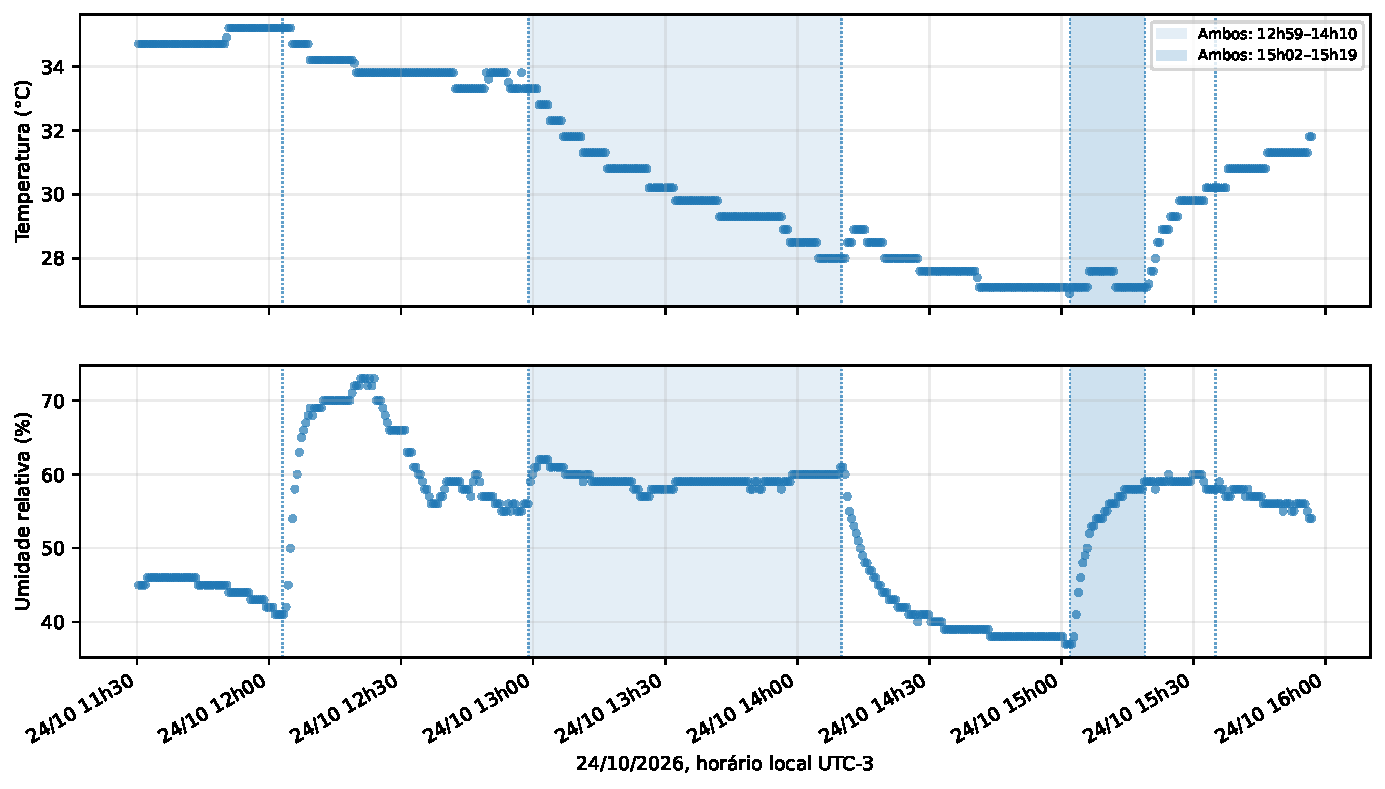
\includegraphics[width=\textwidth]{figuras/ensaio_simultaneo_final.pdf}\caption{Temperatura e umidade medidas na tarde de 24/10. Faixas sombreadas assinalam funcionamento simultâneo; linhas pontilhadas marcam intervenções registradas.}\label{fig:simultaneo}\fonte{3.080 telemetrias únicas do arquivo final e diário de eventos.}\end{figure}
\begin{table}[H]\centering\caption{Fases observadas em 24/10 e seus indicadores descritivos}\label{tab:fases}\scriptsize
\begin{tabular}{@{}L{5.5cm}C{1.25cm}C{2.15cm}C{2.15cm}L{3.2cm}@{}}\toprule
Condição / janela&$n$&Temperatura média&UR média&Observação\\\midrule
Umidificador, 12h03--12h59&112&33,89~\si{\celsius}&62,23\%&Antes do ar\\
Ambos ligados, 12h59--14h10&142&30,14~\si{\celsius}&59,28\%&Ar ajustado a 24~\si{\celsius}\\
Somente ar, 14h10--15h02&104&27,63~\si{\celsius}&41,34\%&Umidificador desligado\\
Ambos ligados, 15h02--15h19&34&27,28~\si{\celsius}&53,32\%&Segundo ensaio\\
Janela aberta e umidificador, 15h19--15h35&32&29,25~\si{\celsius}&59,00\%&Ar desligado; ventilação externa\\
Janela aberta, sem aparelhos, 15h35--15h56&44&30,99~\si{\celsius}&56,57\%&Fim da campanha\\\bottomrule\end{tabular}\fonte{Médias de telemetrias únicas cujos horários de aquisição estão nos intervalos semiabertos assinalados.}\end{table}
As janelas possuem extensões diferentes, e não houve controle de clima externo, potência real dos aparelhos nem distância exata ao sensor. Por isso, a diferença entre as médias das fases não representa efeito causal nem comparação experimental randomizada. Mesmo assim, a marcação temporal dos eventos torna o dataset adequado a rótulos exploratórios como \emph{umidificação isolada}, \emph{refrigeração isolada}, \emph{operação conjunta} e \emph{janela aberta}.
\section{Placar dos requisitos e passagem para a AP3}
Dos 13 requisitos da Tabela~\ref{tab:rastreabilidade}, 11 foram atendidos e 2 atendidos em parte; nenhum ficou sem atender. Os dois parciais são \RNF{05}, porque o nó não valida o certificado do servidor, e \RNF{06}, porque o custo do rádio não foi medido. As etapas de sensoriamento e gravação em CSV funcionaram: foram recebidas 3.082 telemetrias e o analisador identificou 3.080 únicas, com duas duplicações e sem saltos internos nos boots observados. O comando remoto alterou a periodicidade; sessões e reconexões foram demonstradas nos testes; os status retidos e o LWT apresentaram transições visíveis. Em contrapartida, a estimativa energética do rádio não foi aferida e o TLS embarcado não autenticou o certificado do servidor sem CA configurada. A autorização por \emph{blacklist} também é menos restritiva que uma política de negação por padrão. Para a AP3, o conjunto de dados oferece episódios anotados, mas requer coleta em outros dias e ambientes para formar base representativa e verificar generalização.
